
\section{Introduction} 

  \subsection{Image Synthesis in Computer Graphics}

      \begin{frame}\frametitle{Direct and Indirect Illumination}
      \begin{itemize}
      \setlength\itemsep{1.5 em}
      \item Rendering-image synthesis from scene given,
      \begin{itemize}
      \item Geometry of scene
      \item Optical properties of surfaces (BRDF)
      \item Location of light sources
      \end{itemize}
      \item Types of renderer
      \begin{itemize}
      \setlength\itemsep{0.5 em}
      \item Direct illumination
      \item Indirect illumination (global illumination)
      \end{itemize}
      \item Types of indirect illumination renderer
      \begin{itemize}
      \setlength\itemsep{0.5 em}
      \item Ray-tracing
      \item Radiosity (lambertian BRDF)
      \end{itemize}
      \end{itemize}
      \end{frame}



      \begin{frame}\frametitle{Direct and Indirect Illumination}
       \begin{figure}
        \centering
        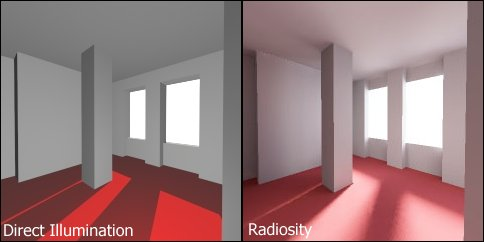
\includegraphics[width=4in]{DirectIndirect.jpg}
        \caption{Direct and Indirect Illumination\footfullcite{www.wikipedia.org/wiki/Radiosity(Computer Graphics)}}
        \label{idealscalable}
        \end{figure}
      \end{frame}



  \subsection{Radiosity Integral Equation (RIE)}


      \begin{frame}\frametitle{Radiosity Integral Equation (RIE)}

      Radiosity $\rightarrow $ Power (light) per unit area
      
      \begin{equation}
      B_i=E_i+\sum_j K_{i,j} B_j, \quad j \in \{All ~ Surfaces\}
      \end{equation}
      
      \centering
      $K_{i,j}=\frac{\text {Radiosity received by i from j}}{\text{Radiosity leaving from j}}$\\
      
      \vspace{2 mm}
      \centering
      $E_i \rightarrow $  Non zero for light source\\
      
      \vspace{2 mm}
      \centering
      $p_i \rightarrow $  BRDF of surface i\\

      \vspace{2 mm}
      \centering
      Domain of surfaces $(M^2)$ is $L^2(\mathbb{R}^2)$ with finite support

      \begin{equation}
      B(x)=E(x)+p(x)\int_{M^2} K(x,y)B(y)dy\quad  \forall ~ x \in M^2
      \end{equation}
      \end{frame}


\section{Literature Survey}

      \begin{frame}\frametitle{Literature Survey}

      \begin{itemize}
      \item Cohen et al. solved with $n$ patches (constant radiosity) and $n^2$ from factors, $K_{i,j}, \quad i,j =1,2,...,n.$

      \item Kajia et al. $\rightarrow$ radiosity integral equation $\rightarrow$ Projection methods (solve RIE in finite dimensional space).

      \item Finite Dimensional space
          \begin{itemize}
          \item Heckbert $\rightarrow$ Piecewise linear 
          \item Zatz $\rightarrow$ Piecewise polynomial of higher order
          \item Hanarahan et al. $\rightarrow$ Hierarchy of basis (Haar wavelet basis)
          \end{itemize}

      \item Gortler et al. $\rightarrow$ used wavelet basis $\rightarrow$ wavelet radiosity

      \end{itemize}
      \end{frame}


\section{Test Scenes and Metric for Comparison}
  \subsection{Radiosity in 2 and 3 Dimensions}


       \begin{frame}\frametitle{Test Scenes: 3 Dimensional}
       \vspace{-0.5 cm}
          \begin{columns}[T]
            \begin{column}{.4\textwidth}
        
    % Your text here
                \begin{figure}
                \centering
                \includegraphics[width=2 in]{3dscene.png}
                \centering
                \caption{3D scene: Two Parallel Surfaces}
                \label{fig_parallel_3D}
                \end{figure}
                

            \end{column}
          \begin{column}{.5\textwidth}
				\vspace{-8 mm}
                \begin{figure}
                \centering
                \includegraphics[width=1.8 in]{xy.png}
                \caption{3D Geometry: Kernel Calculation}
                \label{fig_xy}
                \end{figure}
          \end{column}
        \end{columns}

          \begin{equation} \label{eq:3dkernel}
          K(x,y) =  \frac{\cos \theta_x \cos \theta_y} {\pi r_{xy}^{2}} V(x,y) 
          \end{equation}
          
     
        \end{frame}


  % \subsection{}

      \begin{frame}\frametitle{Test Scenes: 2 Dimensional}
        \begin{columns}[T]
          \begin{column}{.4\textwidth}
      			\vspace{-5 mm}
                \begin{figure}
              \centering
              \captionsetup{justification=centering}

              \includegraphics[width=1.2in]{f1_025.png}
              \vspace{-3 mm}
              \caption{Flatland Scene 1: Parallel Segments}
              \label{fig_parallel}
              \end{figure}
                  

          \end{column}
        \begin{column}{.5\textwidth}

                   \begin{figure}
                \centering
              \captionsetup{justification=centering}

                \includegraphics[width=2in]{f2.png}
                \vspace{-3 mm}
                \caption{Flatland Scene 2: Perpendicular Segments}
                \label{fig_parallel}
                \end{figure}
        \end{column}
      \end{columns}
    \end{frame} 





    \begin{frame}\frametitle{Kernel Calculation: 2 Dimensional }

          \begin{figure}
          \centering
          \includegraphics[width=1.8in]{genken.png}
          \caption{ Kernel for Any Two Line Segments X and Y}
          \label{fig_gen_kernel_2D}
          \end{figure}

          \vspace{-5 mm}

          \begin{equation} \label{eq:2dkernel}
          K(x,y) =  \frac{\cos \theta_x \cos \theta_y} {2 r_{xy}}V(x,y) 
          \end{equation}

    \end{frame}


    \begin{frame}\frametitle{Solution for Flatland Scene 1}
    \vspace{-7 mm}
        
        \begin{columns}[T]
          \begin{column}{.4\textwidth}
      
              \begin{figure}
              \centering
              \includegraphics[width=1.8in]{f1_025_qlmw_scale_b1_plot_n_16.png}
              \vspace{-2 mm}
              \caption{Radiosity $B_1(x)$}
              \label{fig_gen_kernel_2D}
              \end{figure}
        \end{column}

        \begin{column}{.5\textwidth}
              \begin{figure}
              \centering
              \includegraphics[width=1.8in]{f1_025_qlmw_scale_b2_plot_n_16.png}
              \vspace{-2 mm}
              \caption{Radiosity $B_2(y)$}
              \label{fig_gen_kernel_2D}
              \end{figure}
        \end{column}
      \end{columns}
        \begin{columns}[T]
          \begin{column}{.4\textwidth}
      
              \begin{figure}
              \centering
              \includegraphics[width=1.5in]{qlmw_scale_64_025_b1.png}
              \vspace{-2 mm}
              \caption{Image of $B_1$}
              \label{fig_gen_kernel_2D}
              \end{figure}
        \end{column}

        \begin{column}{.5\textwidth}

                \begin{figure}
              \centering
              \includegraphics[width=1.5in]{qlmw_scale_64_025_b2.png}
              \vspace{-2 mm}
              \caption{Image of $B_2$}
              \label{fig_gen_kernel_2D}
              \end{figure}
        \end{column}
      \end{columns}


    \end{frame}

\begin{frame}\frametitle{Solution of Flatland Scene 2}
    \vspace{-7 mm}
      \begin{columns}[T]
          \begin{column}{.4\textwidth}
      
              \begin{figure}
              \centering
              \includegraphics[width=1.8in]{f2_qlmw_scale_b1_plot_n_64.png}
              \vspace{-2 mm}
              \caption{Radiosity $B_1(x)$}
              \label{fig_gen_kernel_2D}
              \end{figure}
        \end{column}

        \begin{column}{.5\textwidth}

                \begin{figure}
              \centering
              \includegraphics[width=1.8in]{f2_qlmw_scale_b2_plot_n_64.png}
              \vspace{-2 mm}
              \caption{Radiosity $B_2(y)$}
              \label{fig_gen_kernel_2D}
              \end{figure}
        \end{column}
      \end{columns}
        \begin{columns}[T]
          \begin{column}{.5\textwidth}
      
              \begin{figure}
              \centering
              \includegraphics[width=1.5in]{f2_qlmw_scale_64_025_b1.png}
              \vspace{-2 mm}
              \caption{Image of $B_1$}
              \label{fig_gen_kernel_2D}
              \end{figure}
        \end{column}

        \begin{column}{.5\textwidth}
              \begin{figure}
              \centering
              \includegraphics[width=1.5in]{f2_qlmw_scale_64_025_b2.png}
              \vspace{-2 mm}
              \caption{Image of $B_2$}
              \label{fig_gen_kernel_2D}
              \end{figure}
        \end{column}
      \end{columns}
    \end{frame}



% \begin{frame}\frametitle{Solution of Flatland scenes 2}
%   \begin{figure}
%   \centering
%   \includegraphics[width=0.5in]{f2_qlmw_scale_64_025_b1.png}
%   \caption{General kernel for two line segments}
%   \label{fig_gen_kernel_2D}
%   \end{figure}
%     \begin{figure}
%   \centering
%   \includegraphics[width=0.5in]{f2_qlmw_scale_64_025_b2.png}
%   \caption{General kernel for two line segments}
%   \label{fig_gen_kernel_2D}
%   \end{figure}
%     \begin{figure}
%   \centering
%   \includegraphics[width=0.5in]{f2_qlmw_scale_b1_plot_n_64.png}
%   \caption{General kernel for two line segments}
%   \label{fig_gen_kernel_2D}
%   \end{figure}
%     \begin{figure}
%   \centering
%   \includegraphics[width=0.5in]{f2_qlmw_scale_b2_plot_n_64.png}
%   \caption{General kernel for two line segments}
%   \label{fig_gen_kernel_2D}
%   \end{figure}

% \end{frame}


  \subsection{Relative Error}

    \begin{frame}\frametitle{Metric for Comparison}
        
        Relative Error in Projection of K
        
        \begin{equation}
        \text{Relative  Error}=\frac{\int\int \,(\,K(x,y)-\hat{K}(x,y)\,)^2  \,dy \, dx}{\int\int \,K(x,y)^2  \,dy \, dx}
        \end{equation}
        
        Relative Error in Projection of B
        
        \begin{equation}
        \text{Relative  Error}=\frac{\int \,(\,B(x)-\hat{B}(x)\,)^2  \,dx}{\int \,B(x)^2  \,dx}
        \end{equation}
    \end{frame}



\section{Projection Methods for Radiosity}

    \begin{frame}\frametitle{Projection Methods for Radiosity}
Discretization of Radiosity Integral Equation, using Basis,$\{N_i(x)\}_{i \in 0,1,2,...}$ ,of the infinite dimensional space $L^2$
\begin{align}
B_p(x) &= \sum_{i=0}^{\infty} \langle B(x),\tilde{N_i}(x) \rangle N_i(x) \\
B_p(x) &= E_p(x)+\int K(x,y)B_p(y) dy \\
B_p(x) &= E_p(x)+ K B_p(x)
\end{align}
~~~~~~~ where, $K B_p(x) = \int K(x,y) B_p(y)dy$
\begin{equation}
K B_p(x) = \sum_{i=0}^{\infty} \langle K B_p(x),\tilde{N_i}(x) \rangle N_i(x) 
\end{equation}

    \end{frame}
    
    \begin{frame}\frametitle{Projection Methods for Radiosity}
    \begin{align}
%\[
\begin{bmatrix}
	B_1 \\
	B_2 \\
	\vdots
\end{bmatrix}
&=
\begin{bmatrix}
	E_1 \\
	E_2 \\
	\vdots
\end{bmatrix}
+
\begin{bmatrix}
    k_{11} & k_{12} & \cdots \\
    k_{21} & k_{22} & \cdots \\
    \vdots & \vdots & \ddots 
\end{bmatrix}
\begin{bmatrix}
	B_1 \\
	B_2 \\
	\vdots
\end{bmatrix}
%\] 
\end{align}

\begin{equation}
\textbf{B} = \textbf{E} + \textbf{K}\textbf{B}
\end{equation}
$K_{i,j}=\langle\, \langle K(x,y),N_j(y)\rangle,\tilde{N}_i(x) \,\rangle =\int \int K(x,y)N_j(y)\tilde{N}_i(x) dy\,dx$

\begin{itemize}
\item Discrete, but countably infinite no. of coefficients
\item Project in finite dimensional space $\rightarrow$ Finite no. of coefficients
\item Error in Projection $\rightarrow$ Choice of finite dimensional space
\item Speed of solution $\rightarrow$ Choice of a basis for the chosen space
\end{itemize}
    \end{frame}

\begin{frame}\frametitle{Implementation of Algorithm}

\begin{itemize}
\item Select finite dimensional function space 
\item Select Basis for that space
\item Project $E(x)$ and $K(x)$ into chosen space $\rightarrow$ inner product using Gauss-Legendre Quadrature rule for integration
\item Solve System of linear equation using Jacobi iteration
\end{itemize}
Radiosity for scene with RGB colors can be calculated by solving this algorithm for 3 wavelength separately.

\end{frame}
\subsection{Choice of a Finite Dimensional Space}
    \begin{frame}\frametitle{Choice of a Finite Dimensional Space}
        
      Space of piece-wise polynomial functions of order $m$, over standard interval ($1/n$), using set of shifted Legendre polynomial up to order $m$
      \vspace{-7 mm}
      \begin{columns}[T]
         \begin{column}{.5\textwidth}
      
            \begin{figure}
            \centering
            \includegraphics[width=2.5in]{f1_025_error_vs_n_all_three.png}
            \caption{Error in Projection of K(x,y) for Flatland Scene 1}
            \label{fig_e_vs_n_f1}
            \end{figure}
        \end{column}
         \begin{column}{.5\textwidth}

            \begin{figure}
            \centering
            \includegraphics[width=2.5in]{f2_025_error_vs_n_all_three.png}
            \caption{Error in Projection of K(x,y) for Flatland Scene 2}
            \label{fig_e_vs_n_f2}
            \end{figure}
        \end{column}
        \end{columns}
\end{frame}




\begin{frame}\frametitle{Analytical Solution}
\begin{equation}
  B(x)=1+\int K(x,y)B(y)dy
\end{equation}
\centering
$  K(x,y)=x^2+xy, \quad x,y \in [0,1]$\\
\centering
Degenerate kernel, $K(x,y) = \sum\limits_{i=1}^na_i(x)b_i(y) $
 
%      \begin{columns}[T]
%         \begin{column}{.5\textwidth}
%
%              \begin{figure}
%              \centering
%              \includegraphics[width=1.5 in]{ahaar4.png}
%              \caption{Solution using\\ $n=4,m=0$}
%              \label{fig_e_vs_n_f1}
%              \end{figure}
%        \end{column}
%         \begin{column}{.5\textwidth}
%
%              \begin{figure}
%              \centering
%              \includegraphics[width=1.5 in]{ahaar16.png}
%              \caption{Solution using $n=16,m=0$}
%              \label{fig_e_vs_n_f2}
%              \end{figure}
%        \end{column}
%        \end{columns}
\end{frame}

\begin{frame}\frametitle{Numerical Solution with $m = 0$}
 \begin{columns}[T]
         \begin{column}{.5\textwidth}

              \begin{figure}
              \centering
              \includegraphics[width=2.5 in]{ahaar4.png}
              \caption{Solution Using \\ $n=4,m=0$}
              \label{fig_e_vs_n_f1}
              \end{figure}
        \end{column}
         \begin{column}{.5\textwidth}

              \begin{figure}
              \centering
              \includegraphics[width=2.5 in]{ahaar16.png}
              \caption{Solution Using \\ $n=16,m=0$}
              \label{fig_e_vs_n_f2}
              \end{figure}
        \end{column}
        \end{columns}

\end{frame}



    \begin{frame}\frametitle{Numerical Solution with $m=1$}
    
      \begin{columns}[T]
        \begin{column}{.5\textwidth}
      
    % Your text here
              \begin{figure}
              \centering
              \includegraphics[width=2.5in]{allmw2.png}
              \caption{Solution Using \\ $n=2,m=1$}
              \label{fig_e_vs_n_f1}
              \end{figure}

        \end{column}
      \begin{column}{.5\textwidth}

              \begin{figure}
              \centering
              \includegraphics[width=2.5in]{allmw4.png}
              \caption{Solution Using \\ $n=4,m=1$}
              \label{fig_e_vs_n_f2}
              \end{figure}

      \end{column}
    \end{columns}
    \end{frame}

\begin{frame}\frametitle{Numerical Solution with $m = 2$}



    \begin{columns}[T]
      \begin{column}{.5\textwidth}
      
              % Your text here
              \begin{figure}
              \centering
              \includegraphics[width=2.5in]{aqlmw1.png}
              \caption{Solution Using \\ $n=1,m=2$}
              \label{fig_e_vs_n_f1}
              \end{figure}

      \end{column}
      \begin{column}{.5\textwidth}
              \begin{figure}
              \centering
              \includegraphics[width=2.5in]{aqlmw2.png}
              \caption{Solution Using \\ $n=2,m=2$}
              \label{fig_e_vs_n_f2}
              \end{figure}

        \end{column}
      \end{columns}
    \end{frame}


  \subsection{Choice of a Basis}

    \begin{frame}
    \frametitle{Choice of a Basis: Wavelets}
    Choice of alternative basis for chosen space
        \begin{itemize}
        \item Haar
        \item Linear Legendre Multi-Wavelet
        \item Quadratic Legendre Multi-Wavelet
        \end{itemize}

     Advantages
        \begin{itemize}
        \item Vanishing moments
        \item Negligible coefficients
        \item Sparse system of equation
        \item Faster solution
        \end{itemize}
    \end{frame}

% \\section{choice of basis} % (fold)
% \label{sec:choice_of_basis}

% % section choice_of_basis (end)
    \begin{frame}
    \frametitle{Haar Wavelet: As a Alternate Basis}
    \vspace{-2 mm}
          \begin{columns}[T]
            \begin{column}{.5\textwidth}

                \begin{equation}\label{eq:qlmwphi0}
                \phi_0(x)=
                \left\{
                    \begin{array}{ll}
                        1  ~~~~  \mbox{if } 0 \leq x < 1 \\
                        0 ~~~~  elsewhere
                    \end{array}
                \right.
                \nonumber
                \end{equation}

        \end{column}
        \begin{column}{.5\textwidth}

              \begin{equation}
              \psi_0(x)=
              \left\{
                  \begin{array}{ll}
                      1 ~~~~~~  \mbox{if } 0 \leq x < \frac{1}{2} \\
                      -1 ~~~~  \mbox{if } \frac{1}{2} \leq x < 1 \\
                      0 ~~~~~~  elsewhere
                  \end{array}
              \right.
              \nonumber
              \end{equation}

        \end{column}
      \end{columns}

        \vspace{9 mm}

          \begin{columns}[T]
            \begin{column}{.5\textwidth}
                
                 Basis: Haar scaling function 
        \vspace{0.5cm}

                 \centering
                  $\{  \phi_{\frac{1}{n},k}(x)\}$,\\
        \vspace{0.2cm}

                   $k=0,1,...,n-1$\\
        \vspace{0.5cm}

                  where, 
                  $\phi_{\frac{1}{n},k}(x)={\sqrt{n}}\phi_0(nx-k)$

        \end{column}
        \begin{column}{.5\textwidth}
                 Basis: Haar wavelet 

            \vspace{0.5cm}

                 \centering
                  $\{ \phi_0(x),\psi_0(x), \psi_{\frac{1}{L},k}(x)\}$,\\ \vspace{0.2cm}
                   $L=2,4,8,...,2^{n-1}$ and $k=0,1,...,L-1$\\
        \vspace{0.5cm}
                  
                  where, 
                  $\psi_{\frac{1}{n},k}(x)={\sqrt{n}}\psi_0(nx-k)$

        \end{column}
      \end{columns}

    \end{frame}


\section{Experiments and Results}


\begin{frame}\frametitle{Sparsity of Kernel Projection Matrix}
Flatland 1 using Haar wavelet and scaling functions.
Radius of circle is proportional to  absolute value of coefficient 


    \begin{columns}[T]
      \begin{column}{.5\textwidth}
      
              % Your text here
              \begin{figure}
              \centering
              \includegraphics[width=1.8in]{res/haarscale16025.png}
              \caption{Scaling Functions as basis}
              \label{fig_e_vs_n_f1}
              \end{figure}

      \end{column}
      \begin{column}{.5\textwidth}
              \begin{figure}
              \centering
              \includegraphics[width=1.8in]{res/haarwavelet16_f2.png}
              \caption{Wavelet Functions as basis}
              \label{fig_e_vs_n_f2}
              \end{figure}

        \end{column}
      \end{columns}
\end{frame}


\begin{frame}\frametitle{Linear Legendre Multi-wavelet (LLMW)}
Two mother wavelet and scaling function
    \begin{columns}[T]
      \begin{column}{.5\textwidth}
      
              % Your text here
              \begin{figure}
              \centering
              \includegraphics[width=1.8in]{llmwphi0.png}
              \caption{LLMW: $\phi^0(x)$}
              \label{fig_e_vs_n_f1}
              \end{figure}
              \tiny{

              \begin{equation}
              \phi^0(x)=
              \left\{
                  \begin{array}{ll}
                      1  & \mbox{if } 0 \leq x < 1 \\
                      0 & elsewhere
                  \end{array}
              \right.
              \nonumber
              \end{equation}}



      \end{column}
      \begin{column}{.5\textwidth}
              \begin{figure}
              \centering
              \includegraphics[width=1.8in]{llmwphi1.png}
              \caption{LLMW: $\phi^1(x)$}
              \label{fig_e_vs_n_f2}
              \end{figure}
              % \vspace{-9 mm}
              \tiny{

              \begin{equation}
              \phi^1(x)=
              \left\{
                  \begin{array}{ll}
                      \sqrt{3}(2x-1)  & \mbox{if } 0 \leq x < 1 \\
                      0 & elsewhere
                  \end{array}
              \right.
              \nonumber
              \end{equation}}
        \end{column}
      \end{columns}
\end{frame}

\begin{frame}\frametitle{Linear Legendre Multi-wavelet (LLMW)}

    \begin{columns}[T]
      \begin{column}{.5\textwidth}
      
              % Your text here
              \begin{figure}
              \centering
              \includegraphics[width=1.8in]{llmwpsi0.png}
              \caption{LLMW: $\psi^0(x)$}
              \label{fig_e_vs_n_f1}
              \end{figure}
              \vspace{-4 mm}

              \tiny{
              
              \begin{equation}
              \psi^0(x)=
              \left\{
                  \begin{array}{ll}
                      -\sqrt{3}(4x-1)  & \mbox{if } 0 \leq x < \frac{1}{2} \\
                      \sqrt{3}(4x-1)  & \mbox{if } \frac{1}{2} \leq x < 1 \\
                      0 & elsewhere
                  \end{array}
              \right.
              \nonumber
              \end{equation}}


      \end{column}
      \begin{column}{.5\textwidth}
              \begin{figure}
              \centering
              \includegraphics[width=1.8in]{llmwpsi1.png}
              \caption{LLMW: $\psi^1(x)$}
              \label{fig_e_vs_n_f2}
              \end{figure}

              \tiny{
                            \begin{equation}
                            \psi^1(x)=
                            \left\{
                                \begin{array}{ll}
                                    (6x-1)  & \mbox{if } 0 \leq x < \frac{1}{2} \\
                                    (6x-5)  & \mbox{if } \frac{1}{2} \leq x < 1 \\
                                    0 & elsewhere
                                \end{array}
                            \right.
                            \nonumber
                            \end{equation}}
        \end{column}
      \end{columns}
\end{frame}


\begin{frame}\frametitle{Quadratic Legendre Multi-wavelet (QLMW)}
Three mother wavelet and scaling function

    \begin{columns}[T]
      \begin{column}{.5\textwidth}
      
              % Your text here
              \begin{figure}
              \centering
              \includegraphics[width=1.8in]{qlmwphi0.png}
              \caption{QLMW: $\phi^0(x)$}
              \label{fig_e_vs_n_f1}
              \end{figure}
              \vspace{-4 mm}

              \tiny{
                \begin{equation}\label{eq:qlmwphi0}
                \phi^0(x)=
                \left\{
                    \begin{array}{ll}
                        1  & \mbox{if } 0 \leq x < 1 \\
                        0 & elsewhere
                    \end{array}
                \right.
              \nonumber
              \end{equation}}


      \end{column}
      \begin{column}{.5\textwidth}

              \begin{figure}
              \centering
              \includegraphics[width=1.8in]{qlmwphi1.png}
              \caption{QLMW: $\phi^1(x)$}
              \label{fig_e_vs_n_f2}
              \end{figure}
              \vspace{-4 mm}

              \tiny{
                 \begin{equation}\label{eq:qlmwphi1}
                  \phi^1(x)=
                  \left\{
                      \begin{array}{ll}
                          \sqrt{3}(2x-1)  & \mbox{if } 0 \leq x < 1 \\
                          0 & elsewhere
                      \end{array}
                  \right.
              \nonumber
              \end{equation}}
        \end{column}
      \end{columns}
\end{frame}

\begin{frame}\frametitle{Quadratic Legendre Multi-wavelet (QLMW)}

    \begin{columns}[T]
      \begin{column}{.5\textwidth}
      
              % Your text here
              \begin{figure}
              \centering
              \includegraphics[width=1.8in]{qlmwphi2.png}
              \caption{QLMW: $\phi^2(x)$}
              \label{fig_e_vs_n_f1}
              \end{figure}
              \vspace{-4 mm}

              \tiny{
                  \begin{equation}\label{eq:qlmwphi2}
                  \phi^2(x)=
                  \left\{
                      \begin{array}{ll}
                          \sqrt{5}(6x^2-6x+1),  & \mbox{if } 0 \leq x < 1 \\
                          0 & elsewhere
                      \end{array}
                  \right.
              \nonumber
              \end{equation}}


      \end{column}
      \begin{column}{.5\textwidth}
              \begin{figure}
              \centering
              \includegraphics[width=1.8in]{qlmwpsi0.png}
              \caption{QLMW: $\psi^0(x)$}
              \label{fig_e_vs_n_f2}
              \end{figure}
              \vspace{-4 mm}

              \tiny{
                         \begin{equation}
                            \psi^0(x)=
                            \left\{
                                \begin{array}{ll}
                                    -\frac{1}{3}(120x^2-72x+7)  & \mbox{if } 0 \leq x < \frac{1}{2} \\
                                    \frac{1}{3}(120x^2-168x+55)  & \mbox{if } \frac{1}{2} \leq x < 1 \\
                                    0 & elsewhere
                                \end{array}
                            \right.
                            \nonumber
                            \end{equation}}
        \end{column}
      \end{columns}
\end{frame}

\begin{frame}\frametitle{Quadratic Legendre Multi-wavelet (QLMW)}

    \begin{columns}[T]
      \begin{column}{.5\textwidth}
      
              % Your text here
              \begin{figure}
              \centering
              \includegraphics[width=1.8in]{qlmwpsi1.png}
              \caption{QLMW: $\psi^1(x)$}
              \label{fig_e_vs_n_f1}
              \end{figure}
              \vspace{-4 mm}

              \tiny{
                     \begin{equation}
                  \psi^1(x)=
                  \left\{
                      \begin{array}{ll}
                          \sqrt{3}(30x^2-14x+1)  & \mbox{if } 0 \leq x < \frac{1}{2} \\
                          \sqrt{3}(30x^2-46x+17)  & \mbox{if } \frac{1}{2} \leq x < 1 \\
                          0 & elsewhere
                      \end{array}
                  \right.
              \nonumber
              \end{equation}}


      \end{column}
      \begin{column}{.5\textwidth}
              \begin{figure}
              \centering
              \includegraphics[width=1.8in]{qlmwpsi2.png}
              \caption{QLMW: $\psi^2(x)$}
              \label{fig_e_vs_n_f2}
              \end{figure}
              \vspace{-4 mm}

              \tiny{
                        \begin{equation}
                        \psi^2(x)=
                        \left\{
                            \begin{array}{ll}
                                -\frac{\sqrt{5}}{3}(48x^2-18x+1)  & \mbox{if } 0 \leq x < \frac{1}{2} \\
                                \frac{\sqrt{5}}{3}(48x^2-78x+31)  & \mbox{if } \frac{1}{2} \leq x < 1 \\
                                0 & elsewhere
                            \end{array}
                        \right.
                            \nonumber
                            \end{equation}}
        \end{column}
      \end{columns}
\end{frame}

\begin{frame}\frametitle{Sparsity of Kernel Projection Matrix}
Flatland 1 using Haar wavelet and scaling functions
\vspace{-2 mm}
 \begin{figure}
              \centering
              \includegraphics[width=3in]{res/f1_025_haar_scale_distri_n_16.png}
              \vspace{-2 mm}
              \caption{Sorted Coefficients Based on Magnitude}
              \label{fig_e_vs_n_f1}
              \end{figure}
\end{frame}

\begin{frame}\frametitle{Sparsity of Kernel Projection Matrix}
Flatland 1 using LLMW wavelet and scaling functions
\vspace{-2 mm}
 \begin{figure}
              \centering
              \includegraphics[width=3in]{res/f1_025_llmw_scale_distri_n_16.png}
              \vspace{-2 mm}
              \caption{Sorted Coefficients Based on Magnitude}
              \label{fig_e_vs_n_f1}
              \end{figure}
\end{frame}

\begin{frame}\frametitle{Sparsity of Kernel Projection Matrix}
Flatland 1 using LLMW wavelet and scaling functions
\vspace{-2 mm}
 \begin{figure}
              \centering
              \includegraphics[width=3in]{res/f1_025_llmw_scale_distri_n_16_log.png}
              \vspace{-2 mm}
              \caption{Sorted Coefficients Based on Magnitude (Log Scale)}
              \label{fig_e_vs_n_f1}
              \end{figure}
\end{frame}

\begin{frame}\frametitle{Sparsity of Kernel Projection Matrix}
Flatland 1 using QLMW wavelet and scaling functions
\vspace{-2 mm}
 \begin{figure}
              \centering
              \includegraphics[width=3in]{res/f1_025_qlmw_scale_distri_n_16_log.png}
              \vspace{-2 mm}
              \caption{Sorted Coefficients Based on Magnitude (Log Scale)}
              \label{fig_e_vs_n_f1}
              \end{figure}
\end{frame}


\begin{frame}\frametitle{Error in Projection}
Keeping top n coefficients (rest of the coefficient are set to zero)
\vspace{-2 mm}
 \begin{figure}
              \centering
              \includegraphics[width=3in]{res/topn256haarbothf1_log_log.png}
              \vspace{-2 mm}
              \caption{Haar, $n = 256$}
              \label{fig_e_vs_n_f1}
              \end{figure}
\end{frame}

\begin{frame}\frametitle{Error in Projection}
Keeping top n coefficients (rest of the coefficient are set to zero)
\vspace{-2 mm}
 \begin{figure}
              \centering
              \includegraphics[width=3in]{res/64topnllmwf1both_log_log.png}
              \vspace{-2 mm}
              \caption{LLMW, $n = 64$}
              \label{fig_e_vs_n_f1}
              \end{figure}
\end{frame}



\begin{frame}\frametitle{Image Synthesis from 3D scene: Haar Wavelet}
% Keeping top n coefficients (rest of the coefficient are set to zero)
Solution of 3D scene with Haar wavelet and $n=4$
\vspace{-2 mm}
 \begin{figure}
              \centering
              \includegraphics[width=4in]{res/3dhaar4_025.png}
              \vspace{-2 mm}
              \caption{Illumination of 3D scene (2 parallel surfaces) by square light source shown near center of one surface (left image)}
              \label{fig_e_vs_n_f1}
              \end{figure}
\end{frame}

\begin{frame}\frametitle{Image Synthesis from 3D scene: Haar Wavelet}
% Keeping top n coefficients (rest of the coefficient are set to zero)
Solution of 3D scene with Haar wavelet and $n=16$

\vspace{-2 mm}
 \begin{figure}
              \centering
              \includegraphics[width=4in]{res/3dhaar16_025.png}
              \vspace{-2 mm}
              \caption{Illumination of 3D scene (2 parallel surfaces) by square light source shown near center of one surface (left image)}
              \label{fig_e_vs_n_f1}
              \end{figure}
\end{frame}

\begin{frame}\frametitle{Image Synthesis from 3D scene: Haar Wavelet}
% Keeping top n coefficients (rest of the coefficient are set to zero)
Solution of 3D scene with Haar wavelet, $n=16$, retaining half of the $256$ coefficients. 

\vspace{-2 mm}
 \begin{figure}
              \centering
              \includegraphics[width=4in]{res/3dhaar16_025.png}
              \vspace{-2 mm}
              \caption{Illumination of 3D scene (2 parallel surfaces) by square light source shown near center of one surface (left image)}
              \label{fig_e_vs_n_f1}
              \end{figure}
\end{frame}

\begin{frame}\frametitle{Image Synthesis from 3D scene: LLMW Wavelet}
% Keeping top n coefficients (rest of the coefficient are set to zero)
Solution of 3D scene with LLMW wavelet and $n=16$

\vspace{-2 mm}
 \begin{figure}
              \centering
              \includegraphics[width=4in]{res/3dllmw16_025.png}
              \vspace{-2 mm}
              \caption{Illumination of 3D scene (2 parallel surfaces) by square light source shown near center of one surface (left image)}
              \label{fig_e_vs_n_f1}
              \end{figure}
\end{frame}

\begin{frame}\frametitle{Image Synthesis from 3D scene: LLMW Wavelet}
% Keeping top n coefficients (rest of the coefficient are set to zero)
Solution of 3D scene with LLMW wavelet and $n=16$, retaining quarter of the 1024 coefficients.

\vspace{-2 mm}
 \begin{figure}
              \centering
              \includegraphics[width=4in]{res/3dllmw16_025.png}
              \vspace{-2 mm}
              \caption{Illumination of 3D scene (2 parallel surfaces) by square light source shown near center of one surface (left image)}
              \label{fig_e_vs_n_f1}
              \end{figure}
\end{frame}


\begin{frame}\frametitle{Image Synthesis from 3D scene: QLMW Wavelet}
% Keeping top n coefficients (rest of the coefficient are set to zero)
Solution of 3D scene with QLMW wavelet and $n=4$.

\vspace{-2 mm}
 \begin{figure}
              \centering
              \includegraphics[width=4in]{res/3dqlmw4_025.png}
              \vspace{-2 mm}
              \caption{Illumination of 3D scene (2 parallel surfaces) by square light source shown near center of one surface (left image)}
              \label{fig_e_vs_n_f1}
              \end{figure}
\end{frame}


\begin{frame}\frametitle{Image Synthesis from 3D scene: QLMW Wavelet}
% Keeping top n coefficients (rest of the coefficient are set to zero)
Solution of 3D scene with LLMW wavelet and $n=16$, retaining half of the 144 coefficients.

\vspace{-2 mm}
 \begin{figure}
              \centering
              \includegraphics[width=4in]{res/3dqlmw4_025.png}
              \vspace{-2 mm}
              \caption{Illumination of 3D scene (2 parallel surfaces) by square light source shown near center of one surface (left image)}
              \label{fig_e_vs_n_f1}
              \end{figure}
\end{frame}



\section{Conclusion and Future Work}
\begin{frame}\frametitle{Conclusion and Future Work}
\begin{itemize}
\item Projection methods are used to solve a radiosity integral equation.

\item Different finite dimensional function space of piecewise polynomials of order $0,1,2$ has been used for projection.
\item Projection error decreases either when order of polynomials is increased or when interval size is decreased.
\item Different basis like Haar wavelet, shifted Legendre polynomials, Legendre multi-wavelet (linear and quadratic) has been used for Comparison. In future other wavelets like Chebyshev multi-wavelet and other polynomial order wavelets can be used. 
\item Wavelet basis gives very sparse system of linear equations. Thus, setting negligible coefficients to zero increases speed of the algorithm.


\end{itemize}
\end{frame}
\begin{frame}
\begin{itemize}

\item Different test scenes, 2D and 3D, has been used to test the algorithm. In future we can use more test scenes to verify results.

\item Test scene under consideration are without occlusion, in future, testing performance of wavelets with scenes having occlusion  can be done 

\end{itemize}
\end{frame}

% \begin{frame}\frametitle{Future Work}

% \end{frame}


\begin{thebibliography}{99}
\providecommand{\url}[1]{{#1}}
\providecommand{\urlprefix}{URL }
\expandafter\ifx\csname urlstyle\endcsname\relax
  \providecommand{\doi}[1]{DOI~\discretionary{}{}{}#1}\else
  \providecommand{\doi}{DOI~\discretionary{}{}{}\begingroup
  \urlstyle{rm}\Url}\fi
\fontsize{9 pt}{11.2}\selectfont

% \bibitem{SVC_overview}
% H. Schwarz, D. Marpe and T. Wiegand, ``Overview of the Scalable Video Coding Extension of the H.264/AVC Standard,'' \emph{IEEE Trans. on CSVT}, 2007.
\bibitem{Goral}
Goral, Cindy M. and Torrance, Kenneth E. and Greenberg, Donald P. and Battaile, Bennett, ``Modeling the Interaction of Light Between Diffuse Surfaces,'' \emph{SIGGRAPH Comput. Graph.}, 1984.

\bibitem{Whitted}
Whitted, Turner, ``An Improved Illumination Model for Shaded Display,'' \emph{Commun. ACM}, June 1980.
\bibitem{Kajiya}
Kajiya, James T., ``The Rendering Equation,'' \emph{SIGGRAPH Comput. Graph.}, Aug. 1986.



% \bibitem{wikiradiosity}
% Wikipedia, ``http://en.wikipedia.org/wiki/Radiosity_(computer_graphics),'' \emph{SIGGRAPH Comput. Graph.}, Aug. 1986.

\bibitem{iesurvey}
 Ilias S., ``A Survey on Solution Methods for Integral Equations,`` \emph{Commun. ACM}, 2008.

\bibitem{ie}
 Yury V. and Yury G. ,``Integral Equations,``2002,


% \bibitem{book:goswami}
%  Goswami, Jaideva C. and Chan, Andrew K.,``Fundamentals of Wavelets: Theory, Algorithms, and Applications,``,2011,isbn = {9780470484135},2nd edition, Wiley Publishing.

\bibitem{book:Stollnitz}
 Stollnitz, Eric J. and Derose, Tony D. and Salesin, David H.,``Wavelets for Computer Graphics: Theory and Applications,``1996, isbn = {1-55860-375-1}, Morgan Kaufmann Publishers Inc..
 % address = {San Francisco, CA, USA},
% } 
\bibitem{book:stoer}
Stoer J. , Bulirsch R.,``Introduction to Numerical Analysis,``1980, Springer Verlag, New York.

\bibitem{iemethod1}
Lakestani, Mehrdad and Saray, Behzad Nemati and Dehghan, Mehdi,``Numerical Solution for the Weakly Singular Fredholm Integro-differential Equations Using Legendre Multiwavelets,``\emph{J. Comput. Appl. Math.}, April, 2011.

\bibitem{iemethod2}
Alpert, Bradley K.,``A Class of Bases in L2 for the Sparse Representations of Integral Operators``,\emph{SIAM J. Math. Anal.}, Jan. 1993.
%  volume = {24},
%  number = {1},
%  month = jan,
%  year = {1993},
%  issn = {0036-1410},
%  pages = {246--262},
%  numpages = {17},
%  url = {http://dx.doi.org/10.1137/0524016},
%  doi = {10.1137/0524016},
%  acmid = {154090},
%  publisher = {Society for Industrial and Applied Mathematics},
%  address = {Philadelphia, PA, USA},
%  keywords = {integral equations, sparse matrices, wavelets},
% } 



\bibitem{hanarahan}
Hanrahan, Pat and Salzman, David and Aupperle, Larry,``A Rapid Hierarchical Radiosity Algorithm``\emph{SIGGRAPH Comput. Graph.}, July 1991.
%  volume = {25},
%  number = {4},
%  month = jul,
%  year = {1991},
%  issn = {0097-8930},
%  pages = {197--206},
%  numpages = {10},
%  url = {http://doi.acm.org/10.1145/127719.122740},
%  doi = {10.1145/127719.122740},
%  acmid = {122740},
%  publisher = {ACM},
%  address = {New York, NY, USA},
%  keywords = {global illumination, n-body problem, radiosity, ray-tracing},
% } 


\bibitem{heckbert}
 Heckbert, Paul Seagrave,``Simulating Global Illumination Using Adaptive Meshing,``, 1992.
%  note = {UMI Order No. GAX92-03586},
%  publisher = {University of California at Berkeley},
%  address = {Berkeley, CA, USA},
% } 


\bibitem{zatz}
 Zatz, Harold R.,``Galerkin Radiosity A Higher Order Solution Method  for Global Illumination,``\emph{SIGGRAPH '93}, 1993.
%  isbn = {0-89791-601-8},
%  location = {Anaheim, CA},
%  pages = {213--220},
%  numpages = {8},
%  url = {http://doi.acm.org/10.1145/166117.166145},
%  doi = {10.1145/166117.166145},
%  acmid = {166145},
%  publisher = {ACM},
%  address = {New York, NY, USA},
%  keywords = {Galerkin methods, curved surfaces, global illumination, integral equations, progressive refinement, radiosity},
% } 
\bibitem{gortler}
Gortler, Steven J. and Schrder, Peter and Cohen, Michael F. and Hanrahan, Pat,``Wavelet Radiosity,``\emph{SIGGRAPH '93}, 1993.

\end{thebibliography}

\begin{frame}[noframenumbering]\frametitle{}

\end{frame}